\chapter{Projetos em CUAD}

Para elaborar projetos com concreto de ultra alto desempenho, é imprescindível ter em mente que as características inerentes do material possibilitam a exploração de novos métodos e geometrias de construção que otimizem e justifiquem seu uso em detrimento dos métodos tradicionais de construção. Apesar disso, com exceção da passarela de Sherbrooke (\autoref{chap:sher}), nenhuma das estruturas feitas com CUAD possuem um projeto topológico drasticamente diferente do utilizado em estruturas de concreto convencional \cite[p.~603]{Flint}.

%\citeonline{Flint} sugerem o uso de algoritmos como ``otimização da colônia da formiga'' que, através de diversas iterações, procura chegar à uma solução ótima de caminho mínimo de distribuição de cargas para um determinado problema estrutural. Aplicando-se outros algoritmos e inteligência artificial também pode ocasionar na descoberta de topologias diferentes e inovadoras que se encaixem na proposta de uso do CUAD e que, de outra maneira, poderiam não ser consideradas pelo projetista. É importante salientar que as soluções computacionais ainda precisam ser interpretadas e desenvolvidas de maneira apropriada por um engenheiro competente.

A computação já inspira arquitetos e engenheiros a desenvolverem soluções de arquitetura e engenharia inovadoras, e o CUAD permite a aplicação desses projetos com muito mais facilidade que o aço, possuindo um desempenho muito próximo, mas com uma grande vantagem: a indústria do aço é muito refinada, e seu processo de produção consome muito mais energia e emite muito mais gases poluentes que a indústria do concreto. Outra vantagem que o CUAD leva sobre o aço é a durabilidade, já que sem um tratamento especial e manutenção cuidadosa, o aço se deteriora rapidamente. Por último, oferece um grande desempenho para estruturas comparativamente leves, não sendo um material exótico como fibra de carbono, por exemplo \cite[p.~11]{Davila}.

Atualmente, o CUAD encontra-se em uma fase experimental de adoção, pois ainda não existe um manual que apresente ao engenheiro de estruturas que critérios e elementos são necessários para projeto, além de exemplos claros de implementação. As informações ainda encontram-se espalhadas e os projetos existentes ainda exigem uma análise cuidadosa, caso a caso, o que muita vezes faz com que o responsável pelo projeto adote soluções mais conservadoras, sub-utilizando a capacidade do material. Ainda é preciso um grande trabalho de pesquisa e divulgação do CUAD para que isso seja produzido para o grande público \cite[p.~13]{Davila}.

Mesmo que o CUAD permita a construção de estruturas mais leves e esbeltas, é preciso ter cuidado com a geometria escolhida, além do cuidado com a deformação da peça, já que o seu módulo de elasticidade é apenas duas vezes maior que o do concreto convencional.

As próximas seções mostram os cuidados necessários para trabalhar com o CUAD e alguns exemplos de obras executadas em CUAD, das primeiras às mais recentes.

%Resplendino
%713 Recomenda fucking ções

%Resplendino fachadas
%405

\section{Métodos construtivos para CUAD}

Para se atingir as altas resistências desejadas no CUAD, é imprescindível um rigoroso controle tecnológico dos materiais utilizados na fabricação do CUAD. A adição de fibras em grandes volumes de concreto é por si só problemática, pois não é possível controlar sua distribuição na mistura e sua correta dispersão é altamente desejável para que elas trabalhem a favor da resistência do concreto, e não se acumulem em apenas um local.

A mistura dos materiais pode ser feita de diversas formas, desde que se observe com cuidado a distribuição das fibras. O próximo passo, crucial para que as resistências desejadas sejam atingidas é a cura do concreto, que deve ser feita em ambiente saturado de vapor e, preferencialmente, sob pressão (cura em autoclave), pois isso irá melhorar ainda mais a resistência do CUAD.

Este processo só pode ser controlado corretamente em um ambiente industrializado, de modo que não se recomenda a utilização de CUAD moldado \textit{in loco}, por conta da dificuldade do controle tecnológico do concreto em um ambiente aberto.

\section{Aplicações}
\label{chap:obras-cad}

\subsection{Passarela de Sherbrooke, Canadá}
\label{chap:sher}

A passarela de Sherbrooke (\autoref{sherbrooke}), construída sobre o rio Magog, na cidade de Quebec, Canadá, foi a primeira estrutura construída inteiramente com concreto de pós reativos (CPR), uma variedade de concreto de ultra alto desempenho (CUAD), sem a utilização de barras de aço. Sua superestrutura consiste de treliças de CPR com com uma resistência característica de 200 MPa confinadas em tubos de aço inoxidável sobre um vão de 60 metros \cite[p.~140]{Aitcin_sher}.

\begin{figure}[htb]
	\caption{\label{sherbrooke}Passarela de Sherbrooke, Quebec, Canadá. Construída em CPR (concreto de pós reativos) sem o uso de barras de aço.}
	\begin{center}
	    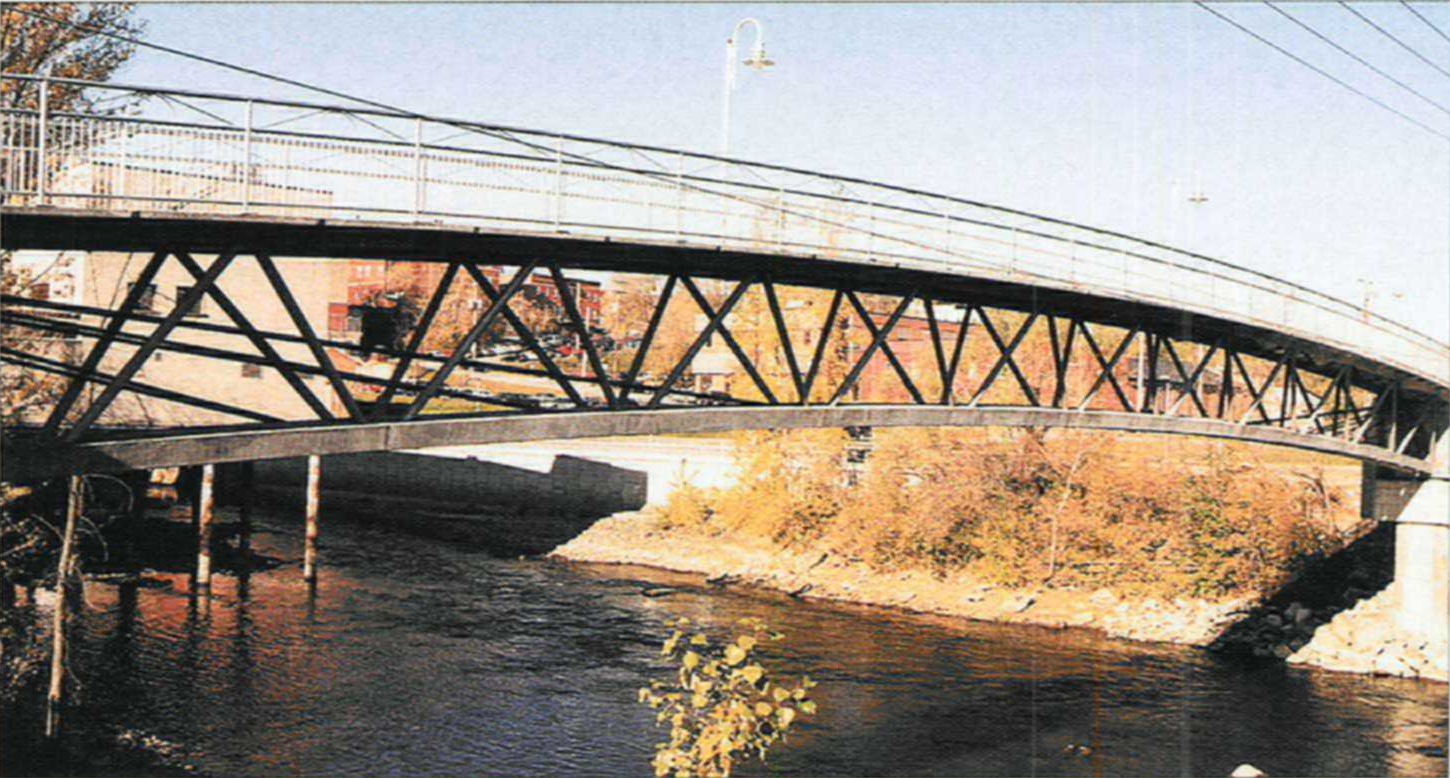
\includegraphics[max width=\textwidth]{sherbrooke.png}
	\end{center}
	\fonte{\citeonline[p.~140]{Aitcin_sher}.}
\end{figure}

As partículas utilizadas no CPR utilizado para construir a passarelas foram limitadas a 0,8 mm. Sua mistura consiste em cimento Portland, fumo de sílica, pó de quartzo, areia, superplastificante, água e fibras de aço com resistência de 2600 MPa, 0,2 mm de diâmetro e 13 mm de comprimento. A mistura foi confinada em tubos de aço inoxidável de 150 mm de diâmetro e espessura de 2 mm. Este confinamento serve para transformar a ruptura frágil apresentada pelo CUAD em uma ruptura pseudo-dúctil, além de melhorar ainda mais as suas propriedades mecânicas, incluindo a  capacidade de suportar uma solicitação de compressão de 350 MPa \citeonline[p.~141]{Aitcin_sher}. A \autoref{sherbrooke_traco} mostra o traço de CPR utilizado na passarela de Sherbrooke. Já a \autoref{sherbrooke_curva} mostra as curvas de tensão-deformação compressivas para diferentes tipos de concretos testados na época da construção da ponte. No gráfico, é possível observar um considerável aumento na resistência à compressão de um mesmo CPR em três condições distintas (livre, confinado e confinado e comprimido). A curva de tensão-deformação do CAD aparece apenas para se fazer um comparativo.

\begin{table}[htb]
\IBGEtab{%
  \caption{Dosagem do CPR usado na passarela de Sherbrooke.}
  \label{sherbrooke_traco}
}{%
  \begin{tabulary}{\linewidth}{CCC}
  \toprule
   Material                 & Quantidade    \\
  \midrule \midrule
   Cimento                  & 705 $\text{kg/m}^3$  \\ \midrule 
   Fumo de sílica           & 230 $\text{kg/m}^3$  \\ \midrule 
   Pó de quartzo            & 210 $\text{kg/m}^3$  \\ \midrule 
   Areia                    & 1010 $\text{kg/m}^3$ \\ \midrule 
   Superplastificante       & 37,5 $\text{l/m}^3$  \\ \midrule 
   Fibras de aço            & 190 $\text{kg/m}^3$  \\ \midrule 
   Água (a/c = 0,21)        & 195 $\text{l/m}^3$   \\
  \bottomrule
\end{tabulary}%
}{%
  \fonte{\citeonline[p.~141]{Aitcin_sher}.}%
  %\nota{Recomenda-se o uso de água de amassamento de baixa temperatura, pré cura térmica de 2 dias e cura térmica de 24 horas a uma temperatura de 80\textsuperscript{\degree} C.}
  %\nota[Anotações]{Uma anotação adicional, que pode ser seguida de várias outras.}
  }
\end{table}

\begin{figure}[htb]
	\caption{\label{sherbrooke_curva} Curvas de tensão-deformação compressivas para diferentes concretos.}
	\begin{center}
	    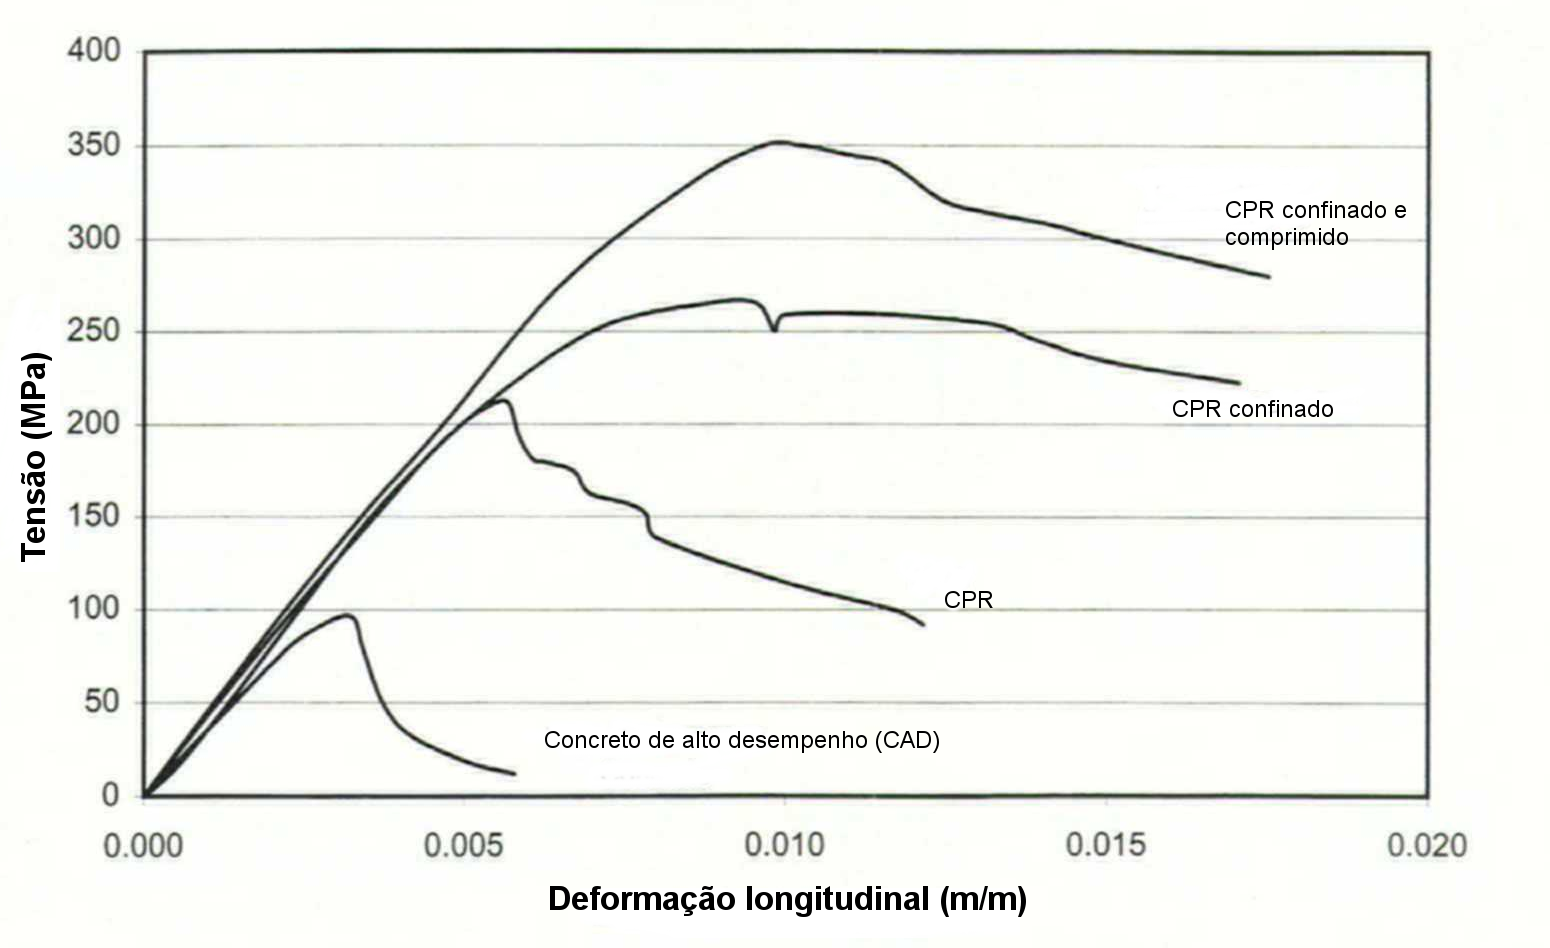
\includegraphics[max width=\textwidth]{sherbrooke-strain.png}
	\end{center}
	\fonte{\citeonline[p.~141]{Aitcin_sher}.}
\end{figure}

Para o projeto da passarela, foram feitas as seguintes considerações: resistência à compressão de 180 MPa, resistência à tração direta de 7 MPa, resistência à flexão de 40 MPa e módulo de elasticidade de 50 GPa. Através de um processo rigoroso de produção introduzido na fábrica de pré-moldados onde a passarela foi moldada, compressão do CPR ainda fresco e cura térmica a vapor, a uma temperatura de 90\textsuperscript{\degree} C, o material foi capaz de atingir uma resistência média de 200 MPa, aferida em corpos de prova recolhidos em diferentes lotes de produção de CPR \cite[p.~141]{Aitcin_sher}.

A passarela possui um tabuleiro de 30 mm de espessura, protendido transversalmente e longitudinalmente e não possui reforço passivo de aço. Por motivos de segurança, o potencial do material não foi explorado completamente, já que esta foi a primeira experiência de uso do material em uma obra aberta ao público \cite[p.~141]{Aitcin_sher}. A seção transversal e longitudinal pode ser vista na \autoref{cross-section} e na \autoref{longitudinal}, respectivamente. A \autoref{precast} mostra um segmento pré-moldado finalizado da ponte, ainda na fábrica.

\begin{figure}[htb]
	\caption{\label{cross-section} Corte transversal da passarela de Sherbrooke.}
	\begin{center}
	    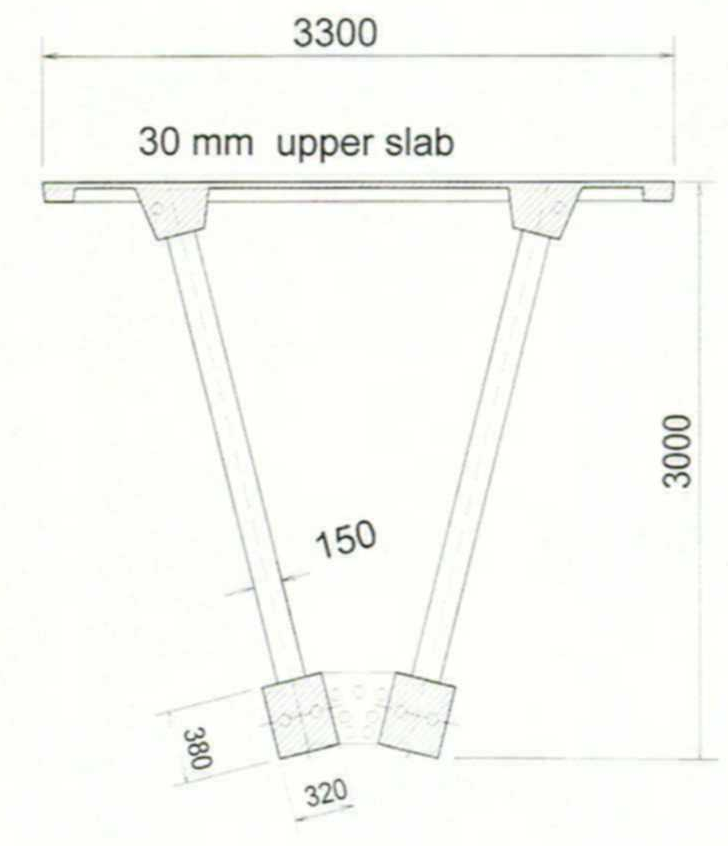
\includegraphics[max width=4cm]{cross-section.png}
	\end{center}
	\fonte{\citeonline[p.~141]{Aitcin_sher}.}
\end{figure}

\begin{figure}[htb]
	\caption{\label{longitudinal}Elevação da passarela de Sherbrooke mostrando a protensão longitudinal.}
	\begin{center}
	    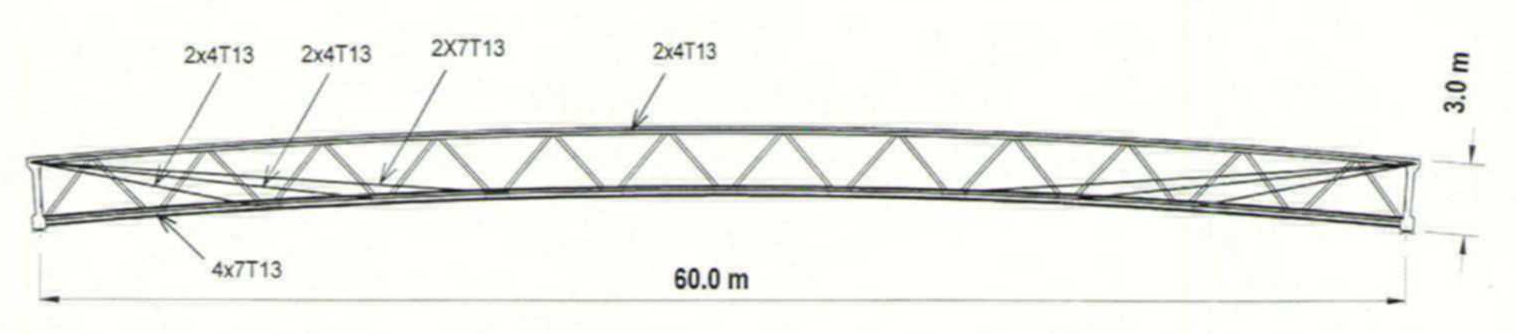
\includegraphics[max width=\textwidth]{longitudinal-prestressing.png}
	\end{center}
	\fonte{\citeonline[p.~142]{Aitcin_sher}.}
\end{figure}

\begin{figure}[htb]
	\caption{\label{precast}Segmento pré-moldado finalizado da passarela.}
	\begin{center}
	    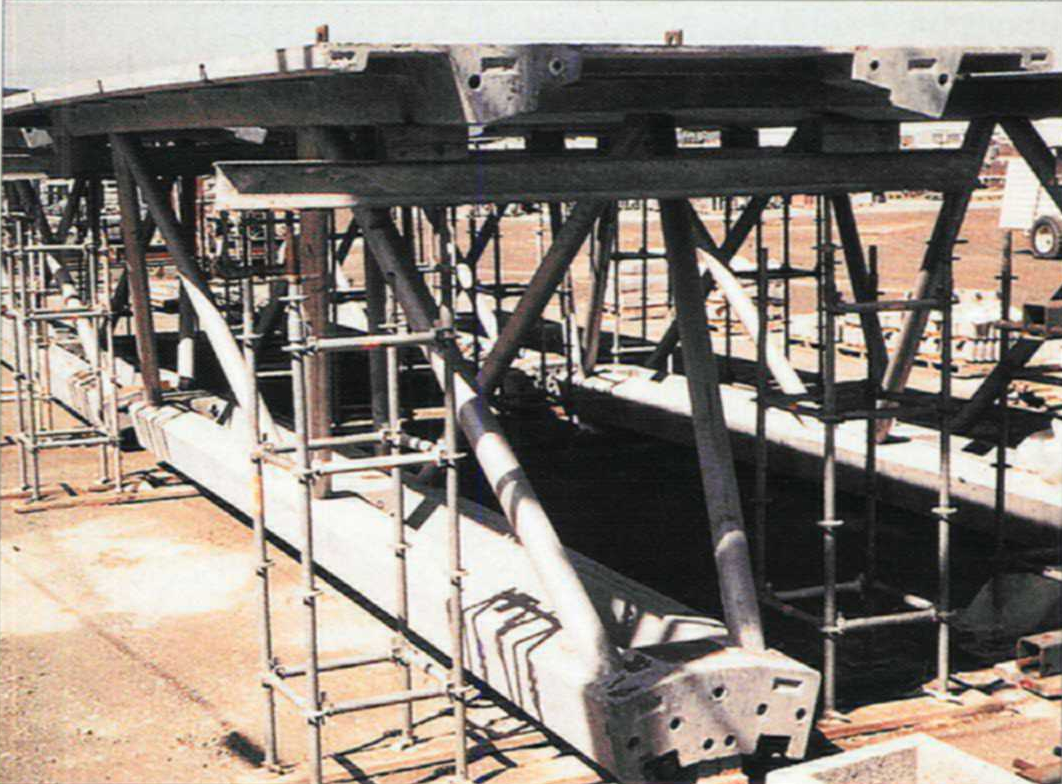
\includegraphics[max width=\textwidth]{precast.png}
	\end{center}
	\fonte{\citeonline[p.~142]{Aitcin_sher}.}
\end{figure}
\subsection{Passarela sobre a ravina de Ovejas, Espanha}

A passarela sobre a ravina de Ovejas, província de Alicante, Espanha é uma passarela de 45 metros (\autoref{ovejas} e \autoref{ovejas-2}), protendida, feita com treliças do tipo Warren de CUAD (\autoref{ovejas-long} e \autoref{ovejas-bottom}). Foi a primeira passarela feita completamente com treliças de CUAD. A espessura do tabuleiro é de apenas 3 cm e a resistência do concreto é de 150 MPa. A \autoref{ovejas-section} e a \autoref{ovejas-section-2} mostram a configuração  da passarela com mais detalhes.

\begin{figure}[htb]
	\caption{\label{ovejas}Passarela sobre a ravina de Ovejas, Província de Alicante, Espanha.}
	\begin{center}
	    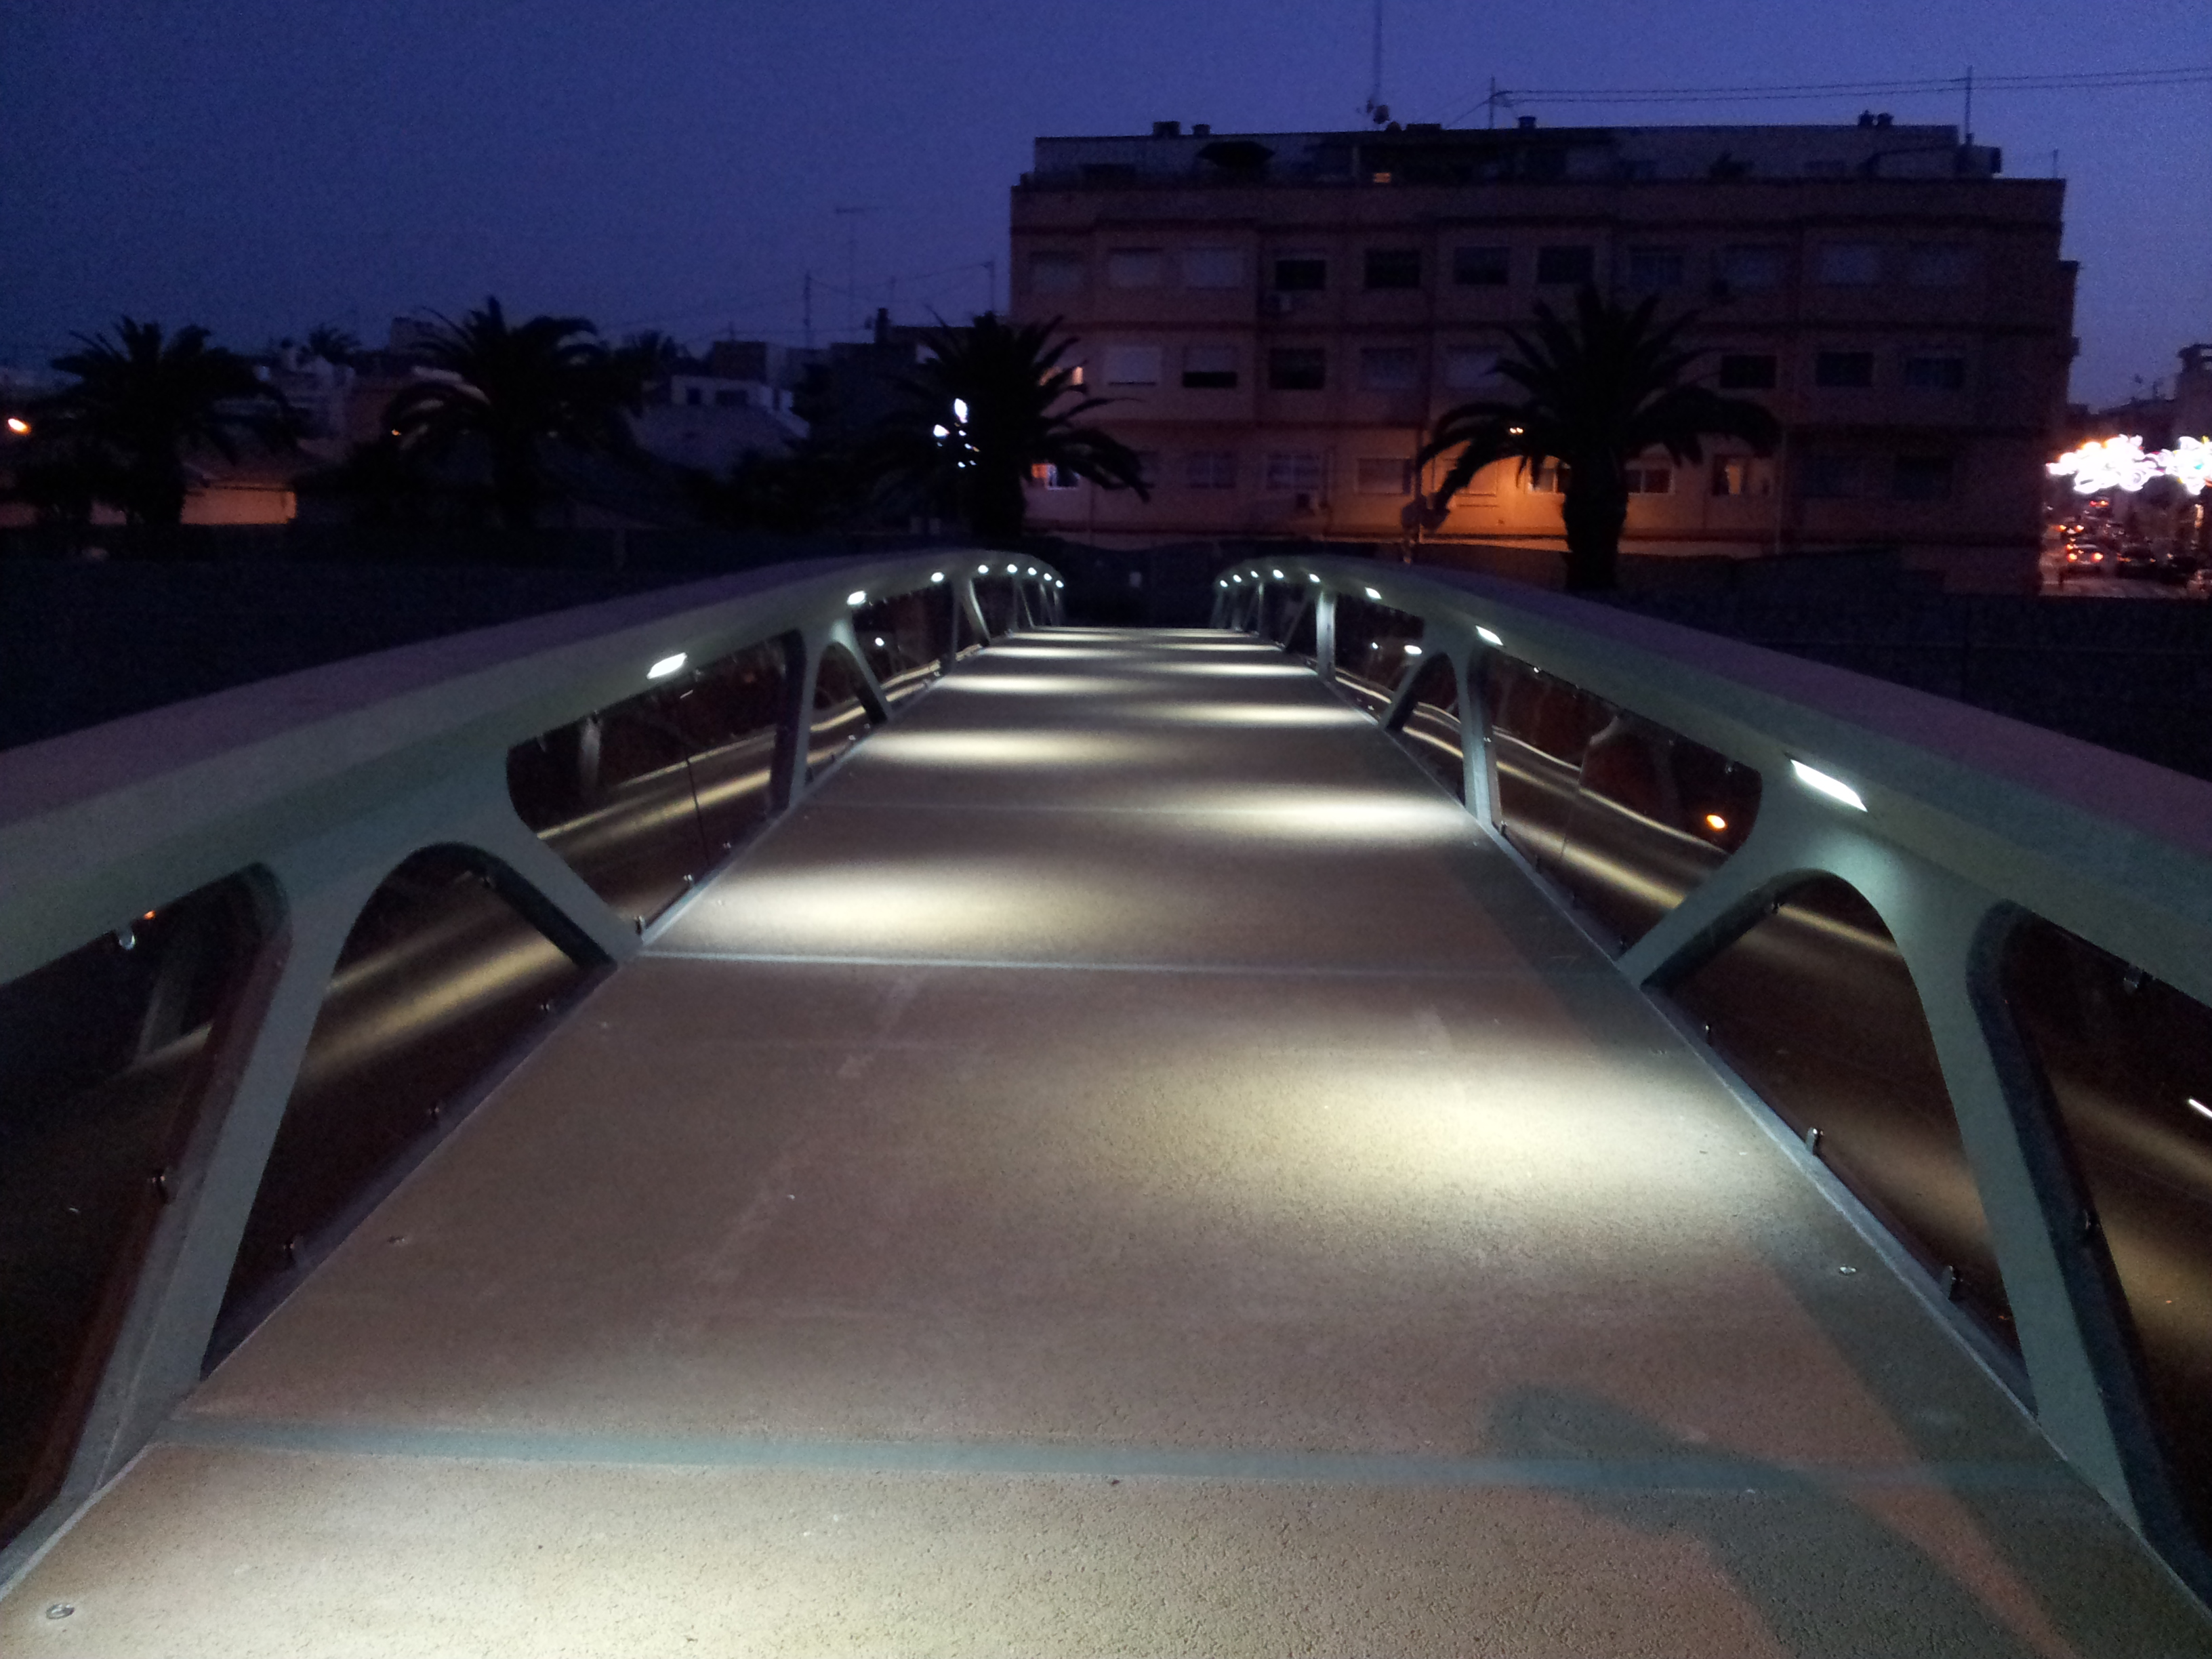
\includegraphics[max width=\textwidth]{passarela-ovejas.jpg}
	\end{center}
	\fonte{\citeonline{RDC}}
\end{figure}

\begin{figure}[htb]
	\caption{\label{ovejas-2}Representação gráfica da passarela de Ovejas.}
	\begin{center}
	    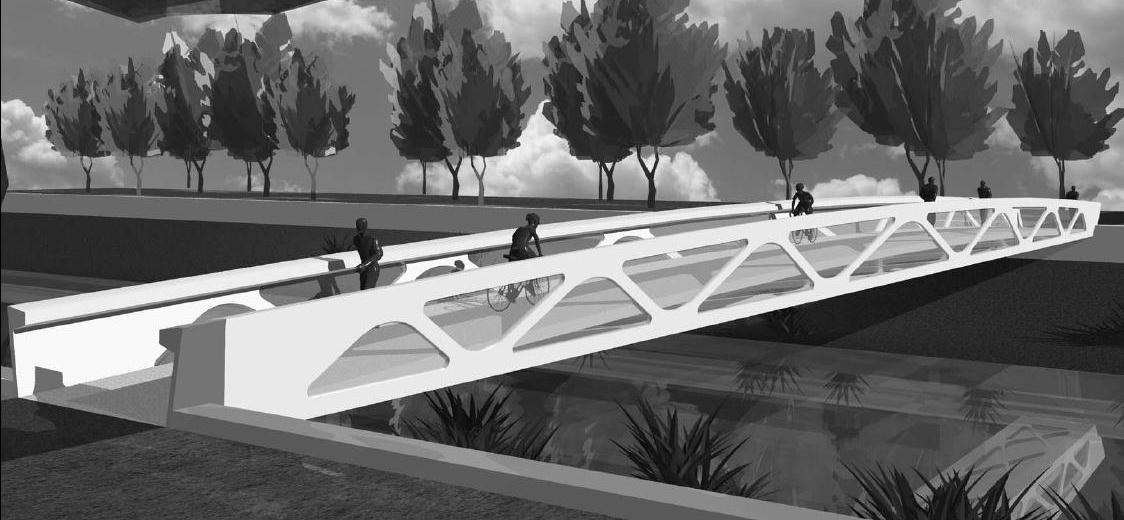
\includegraphics[max width=\textwidth]{ovejas-overview.png}
	\end{center}
	\fonte{\citeonline{Lopez}}
\end{figure}

\begin{figure}[htb]
	\caption{\label{ovejas-long}Vista longitudinal da passarela.}
	\begin{center}
	    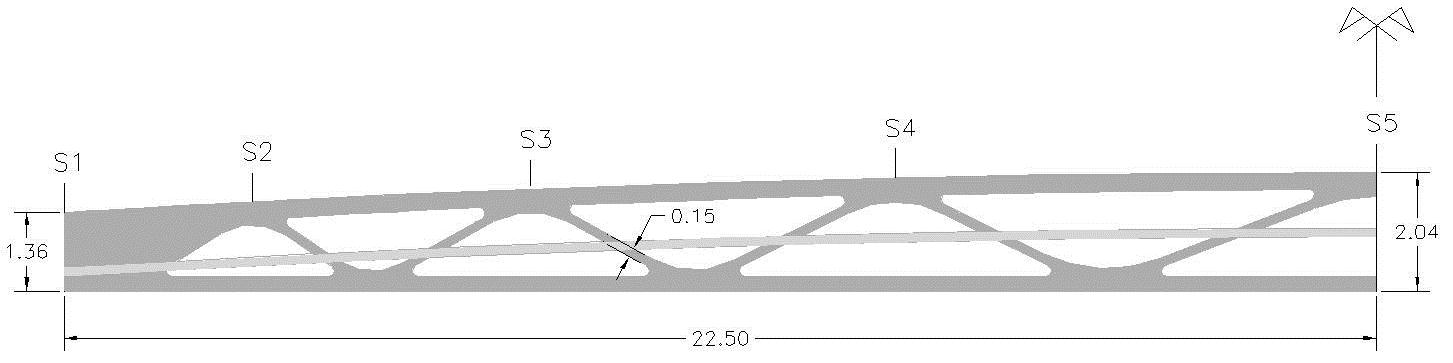
\includegraphics[max width=\textwidth]{ovejas-longitudinal.png}
	\end{center}
	\fonte{\citeonline{Lopez}}
\end{figure}

\begin{figure}[htb]
	\caption{\label{ovejas-bottom}Treliças abaixo do tabuleiro.}
	\begin{center}
	    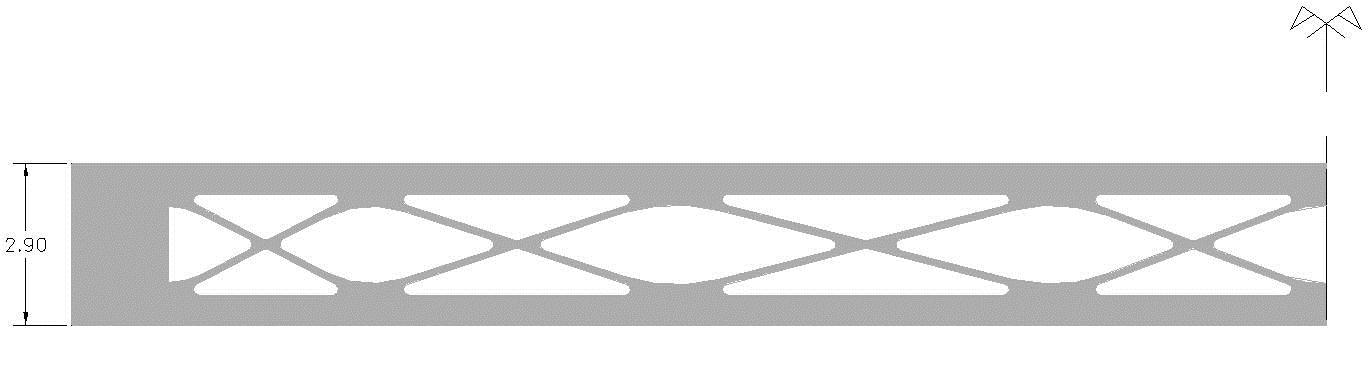
\includegraphics[max width=\textwidth]{ovejas-bottom.png}
	\end{center}
	\fonte{\citeonline{Lopez}}
\end{figure}

\begin{figure}[htb]
	\caption{\label{ovejas-section} Corte transversal da passarela com detalhamento.}
	\begin{center}
	    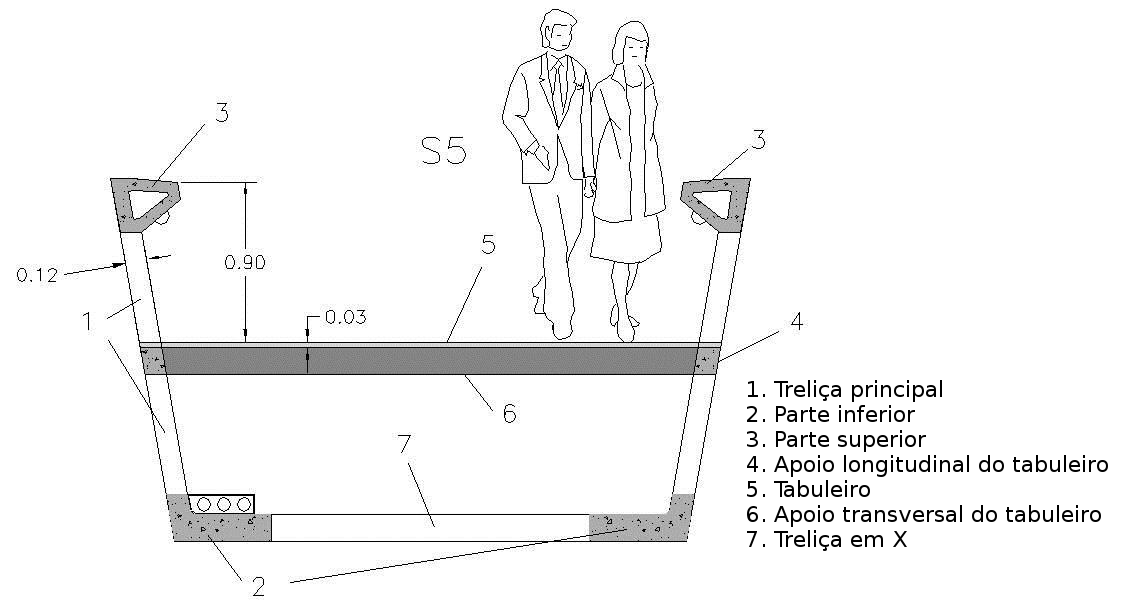
\includegraphics[max width=\textwidth]{ovejas-corte.png}
	\end{center}
	\fonte{\citeonline{Lopez}}
\end{figure}

\begin{figure}[htb]
	\caption{\label{ovejas-section-2}Corte transversal da passarela com detalhamento.}
	\begin{center}
	    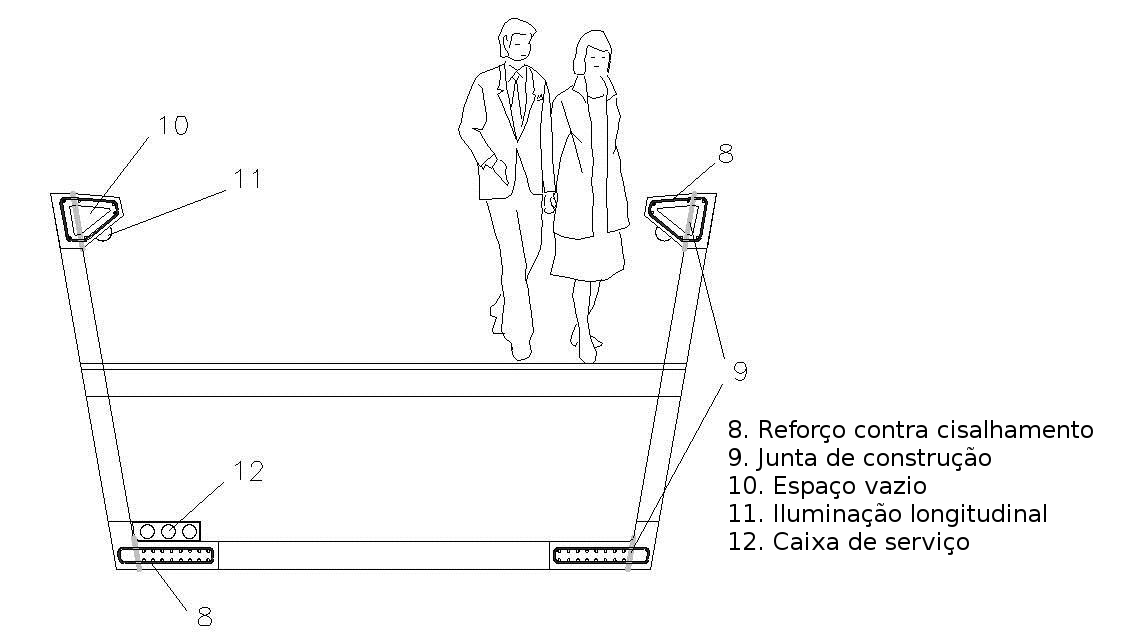
\includegraphics[max width=\textwidth]{ovejas-corte2.png}
	\end{center}
	\fonte{\citeonline{Lopez}}
\end{figure}

A passarela foi moldada na fábrica e transportada por inteiro para sua locação final. O estudo do carregamento da estrutura foi feito com o software SAP2000, considerando as ações especificadas na \autoref{ovejas-acoes}. O traço de concreto utilizado é mostrado na \autoref{ovejas-traco}.


\begin{table}[htb]
	\IBGEtab{%
		\caption{Ações consideradas no projeto da passarela.}
		\label{ovejas-acoes}
		}{%
		\begin{tabulary}{\linewidth}{CC}
			\toprule
			Propriedade                                    & Valor \\
			\midrule \midrule
			Peso próprio                                   & 4,3 kN/m\textsuperscript{2} \\ \midrule
			Carregamento dinâmico característico	       & 5,0 kN/m\textsuperscript{2} \\ \midrule
			Carregamento dinâmico frequente                & 2,0 kN/m\textsuperscript{2} \\ \midrule
			Deformação vertical sob carregamento frequente & 3,6 cm                      \\ \midrule
			Velocidade básica do vento	                   & 18 m/s                      \\ \midrule
			Temperatura mais alta	                       & 34,2\textsuperscript{\degree}C   \\ \midrule
			Temperatura mais baixa                         & 11,5\textsuperscript{\degree}C    \\ \midrule 
			Aceleração sísmica máxima horizontal/vertical  & 3,44/2,41 m/s\textsuperscript{2} \\
			\bottomrule
		\end{tabulary}%
	}{%
	\fonte{\citeonline[p.~899]{Lopez}.}%
			%\nota{Esta é uma nota, que diz que os dados são baseados na regressão linear.}
			%\nota[Anotações]{Uma anotação adicional, que pode ser seguida de várias outras.}
	}
\end{table}

\begin{table}[htb]
	\IBGEtab{%
		\caption{Traço do CUAD utilizado.}
		\label{ovejas-traco}
	}{%
	\begin{tabulary}{\linewidth}{CC}
		\toprule
		Material                                       & Quantidade (kg/m\textsuperscript{3}) \\
		\midrule \midrule
		Cimento (a/c = 0,213)                          & 1000 \\ \midrule
		Fumo de sílica                 	               & 150  \\ \midrule
		Areia 0,5 mm                                   & 702  \\ \midrule
		Areia 1,8 mm                                   & 380  \\ \midrule
		Água                  	                       & 213  \\ \midrule
		Superplastificante \textsuperscript{1}          & 9,06 \\ \midrule
		Fibras OL13/0.16 \textsuperscript{2}            & 78,1 \\ \midrule 
		Fibres RC80/40 BP \textsuperscript{2}           & 78,1 \\
		\bottomrule
	\end{tabulary}%
}{%
\fonte{\citeonline[p.~899]{Lopez}.}%
\nota{\textsuperscript{1)} Fração sólida de superplastificante;}
\nota{\textsuperscript{2)} 1\% em volume de cada fibra de Bekaert.}
%\nota[Anotações]{Uma anotação adicional, que pode ser seguida de várias outras.}
}
\end{table}

%2nd preceedings 45 Ultra-High Performance Concretes – recent realizations and research programs on UHPFRC bridges in France

%2nd preceedings 813 pra frente Muita coisa, não sei se precisa colocar também

%\subsection{Pavimentação}
%1st preceedings 745 Durability and Mechanical Properties of High Performance
%Concrete for Ultra-Thin Whitetopping Pavements

%\subsection{tubos em pontes e prédios}
%1st preceedings 807

%\subsection{Cascas}
%1st preceedings 827 Ultra-High Performance Fibre Reinforced Concret for shells

%2nd preceedings 707 Flexural Behaviour of Fibre Reinforced Ultra High Performance Concrete and the Application in Cladding Panels

\subsection{Ponte Jakway Park}
\label{chap:jakway}

%Para elaborar este estudo de caso, utilizou-se a documentação disponibilizada pelo Departamento de Transporte do estado de Iowa, EUA e pelo e-mail cordialmente enviado pelo engenheiro Brian Keierbeler, com várias informações sobre o projeto da ponte Jakway Park.
%
%Na primeira seção, apresenta-se o processo de concepção do projeto e as motivações que levaram à escolha do CUAD como solução construtiva da ponte. Em seguida, estuda-se uma viga de seção retangular protendida feita com concreto convencional e comparando-a com uma feita em CUAD, calculando a força de protensão inicial exigida em cada uma. Neste trabalho, toma-se a liberdade de extrapolar as equações para cálculo de estruturas de concreto protendido da NBR 6118:2014 para uso em CUAD, já que a própria norma avisa que seus casos de uso são feitos para concretos com $ f_{ck} $ de até 90 MPa. É importante reforçar que ainda não existe normatização para o uso de CUAD em nenhum país, somente as recomendações de uso publicadas pela \cite{AFGC}\footnote{\textit{Association Française de Genie Civil}} e pela \cite{JSCE}\footnote{\textit{Japan Society of Civil Engineers}}, de modo que ainda é preciso desenvolver uma solução própria para cada caso.
%
%Também é importante lembrar que a visita ao empreendimento não foi possível, por conta de se encontrar nos Estados Unidos. Mesmo assim, foi possível observar as características e considerações utilizadas no projeto.
%
%\subsubsection{Características da locação da ponte Jakway Park}

Buchanan, no estado de Iowa, EUA é um município predominantemente rural. \citeonline{Keierleber_email} mostra que as pontes da cidade são muito antigas (muitas construídas entre 1870-1914) e já não são capazes de atender a demanda de veículos atuais. A  \autoref{acidente-1} e a \autoref{acidente-2} retratam acidentes ocorridos no município devido a esta deficiência.

\nomenclature[A]{MIT}{\textit{Massachusetts Institute of Technology}}
\nomenclature[A]{FHWA}{\textit{Federal Highway Administration}}

Como parte de um programa de pesquisa e financiamento através de um programa de construção de pontes inovadoras do governo dos EUA, o município decidiu trocar a velha ponte Jakway Park por uma ponte de CUAD seção $ \pi $, desenvolvida pelo Instituto de Tecnologia de Massachusetts (MIT) e pelo Laboratório Turner-Fairbank da Administração Federal de Rodovias (FHWA) \cite{Keierbeler_et_al}.

\begin{figure}[htb]
	\caption{\label{acidente-1}Acidente em ponte de madeira em Buchanan.}
	\begin{center}
		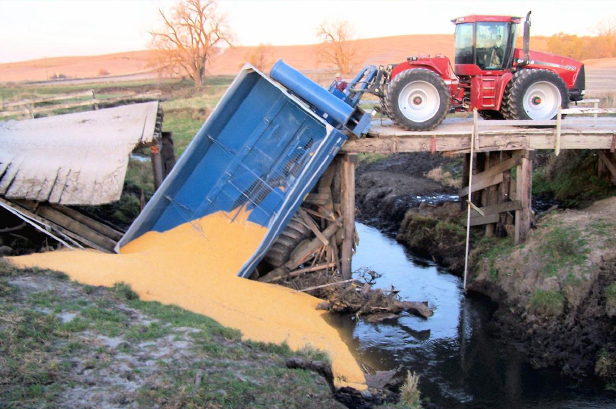
\includegraphics[max width=\textwidth]{acidente-1.png}
	\end{center}
	\fonte{\citeonline{Keierleber_email}}
\end{figure}

\begin{figure}[htb]
	\caption{\label{acidente-2}Acidente em Buchanan.}
	\begin{center}
		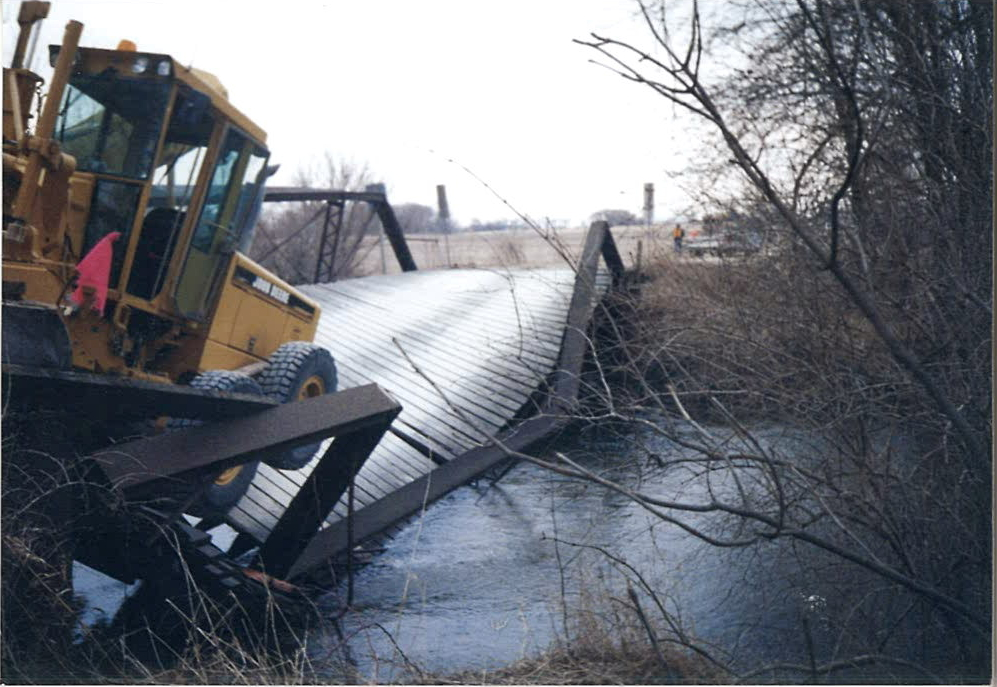
\includegraphics[max width=\textwidth]{acidente-2.jpg}
	\end{center}
	\fonte{\citeonline{Keierleber_email}}
\end{figure}

\subsubsection{Tabuleiro integral de seção \textpi}

O desenvolvimento da seção $ \pi $~começou a ser desenvolvido em 2003 no MIT. O projeto foi otimizado para aproveitar a superior resistência do CUAD para tensão, cisalhamento e compressão, usando a mínima área possível no corte transversal. A primeira geração da seção $ \pi $~(\autoref{secao-pi-1}) falhou nos testes de carregamento, levando os pesquisadores a iterar o projeto \cite[p.~4]{Rouse}. Entre os problemas encontrados, essa geração oferecia um tabuleiro de baixa rigidez, um preocupante comportamento de fissuração com cargas de serviço e problemas na distribuição da carga lateral entre as vigas adjacentes \apud[p.~1]{Graybeal}{Rouse}.

A segunda geração da seção $ \pi $~(\autoref{secao-pi-2}) resolveu os problemas da primeira, sem mudar drasticamente seu desenho, até por questões de economia e reaproveitamento das formas. Com o auxílio do Centro de Engenharia de Pontes (BEC\footnote{\textit{Bridge Engineering Center}}) da Universidade do Estado de Iowa (ISU\footnote{\textit{Iowa State University}}), foi criado um modelo de elementos finitos em 3D no programa ANSYS (\autoref{ansys}). Diversos modelos foram analisados para atender às mudanças necessárias e chegar ao desenho final da nova seção $ \pi $.

Na parte inferior das vigas foi instalado um diafragma metálico, adicionando algum grau de restrição rotacional global no fim das vigas \cite[p.~7]{Rouse}. Cada seção tem uma área de 0,555 m\textsuperscript{2} e um peso próprio de 13,63 kN/m \cite[p.~8]{Rouse}.

Para o dimensionamento das seções que foram utilizadas na construção, limitou-se a resistência a compressão a 148 MPa, por conta do método utilizado para misturar o concreto, o qual foi feito diretamente dentro do caminhão betoneira. Houve o temor que as fibras não se espalhassem da maneira correta, por isso ocorreu essa limitação \cite[p.~8]{Rouse}. A \autoref{valores-de-projeto} lista os dados levados em consideração para o projeto da ponte.

\begin{table}[htb]
	\IBGEtab{%
		\caption{Valores de projeto das propriedades materiais do CUAD.}
		\label{valores-de-projeto}
	}{%
	\begin{tabulary}{\linewidth}{CC}
		\toprule
		Propriedade                                   & Valor (MPa) \\
		\midrule \midrule
		Módulo de elasticidade à liberação            & 39,990 \\ \midrule 
		Módulo de elasticidade final	                 & 53,780 \\ \midrule 
		Resistência de compressão nominal à liberação & 86     \\ \midrule 
		Resistência de compressão nominal final	     & 148    \\ \midrule 
		Resistência nominal à tração final	         & 8,3    \\ \midrule 
		Perda de protensão permitida no escoamento	 & 51,7 (60\% de 86,16 MPa)   \\ \midrule
		Perda de protensão permitida no serviço       & 89   (60\% de 148,33 MPa)  \\ \midrule 
		Tensão de tração permitida no serviço	     & 5,8  (70\% de 8,30 MPa)    \\
		\bottomrule
	\end{tabulary}%
}{%
\fonte{\citeonline[p.~10]{Rouse}.}%
%\nota{Esta é uma nota, que diz que os dados são baseados na regressão linear.}
%\nota[Anotações]{Uma anotação adicional, que pode ser seguida de várias outras.}
}
\end{table}

\begin{figure}[htb]
	\caption{\label{secao-pi-1}Primeira geração da seção $ \pi $.}
	\begin{center}
		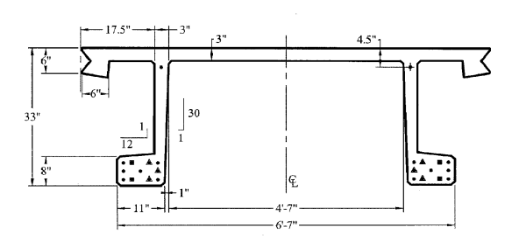
\includegraphics[max width=\textwidth]{secao-pi-1.png}
	\end{center}
	\fonte{\citeonline[p.~5]{Keierleber}}
\end{figure}

\begin{figure}[htb]
	\caption{\label{secao-pi-2}Segunda geração da seção $ \pi $.}
	\begin{center}
		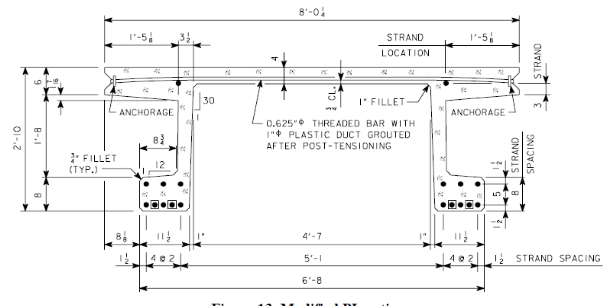
\includegraphics[max width=\textwidth]{secao-pi-2.png}
	\end{center}
	\fonte{\citeonline[p.~10]{Keierleber}}
\end{figure}

\begin{figure}[htb]
	\caption{\label{ansys}Modelo da seção $ \pi $~no ANSYS.}
	\begin{center}
		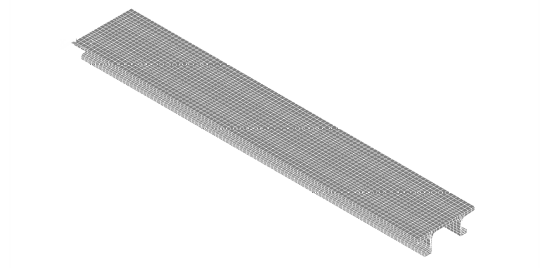
\includegraphics[max width=\textwidth]{ansys.png}
	\end{center}
	\fonte{\citeonline[p.~6]{Rouse}}
\end{figure}

\subsubsection{Construção}

A fornecedora do CUAD utilizado na obra (Lafarge) vende a mistura pronta do concreto. Para fazer o concreto, foi utilizado um caminhão betoneira, misturando o material cimentício, gelo e superplastificantes. Após a homegeinização do concreto, foram adicionadas as fibras de aço com uma peneira, afim de evitar seu agrupamento. Seguiu-se a transferência do CUAD para as formas \autoref{moldagem} e cura térmica a vapor a 90 \textsuperscript{\degree}C por 48 horas (\autoref{vapor}) \cite[p.~17]{Rouse}.

\nomenclature[S]{kN}{Quilonewton}

Em seguida, as peças foram transportadas para o local da construção. As seções adjacentes foram conectadas com barras de 25 mm, posicionadas a cada 45,7 cm e grauteadas (\autoref{corte}, \autoref{detalhe-juntas}  e \autoref{grauteamento}). Para a protensão, foram utilizados 22 cabos de 15 mm de diâmetro (\autoref{protensao}). Desses, 18 foram colocados no bulbo na base das vigas, e tensionados a uma força de 3407 kN. Os outros 4 foram colocados no tabuleiro e tensionados a 756 kN. Difragmas metálicos foram instalados na parte inferior das vigas (\autoref{detalhe-diafragma} e \autoref{foto-diafragma}).

Barras de 15 mm foram posicionadas na parte de baixo do tabuleiro, como reforço de flexão transversal. A instalação foi feita com o auxílio de gruas (\autoref{instalacao}).

A ponte Jakway Park (\autoref{jakway-park}) foi construída num intervalo de 52 dias, sendo inaugurada no dia 26 de novembro de 2008.

\begin{figure}[htb]
	\caption{\label{moldagem}Moldagem da seção $ \pi $.}
	\begin{center}
		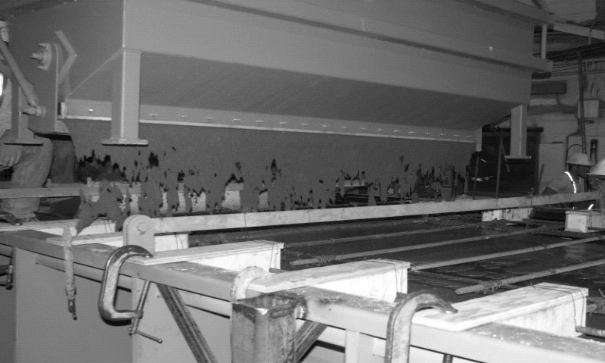
\includegraphics[max width=\textwidth]{moldagem.png}
	\end{center}
	\fonte{\citeonline[p.~17]{Rouse}}
\end{figure}

\begin{figure}[htb]
	\caption{\label{vapor}Cura térmica a vapor.}
	\begin{center}
		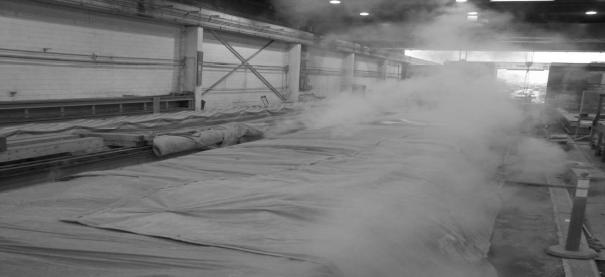
\includegraphics[max width=\textwidth]{vapor.png}
	\end{center}
	\fonte{\citeonline[p.~18]{Rouse}}
\end{figure}

\begin{figure}[htb]
	\caption{\label{corte}Vista em corte.}
	\begin{center}
		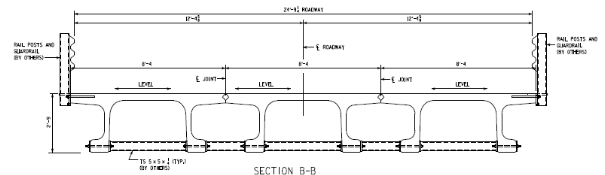
\includegraphics[max width=\textwidth]{corte.png}
	\end{center}
	\fonte{\apudonline[p.~16]{Kei}{Rouse}}
\end{figure}

\begin{figure}[htb]
	\caption{\label{detalhe-juntas}Detalhamento das juntas longitudinais da seção $ \pi $.}
	\begin{center}
		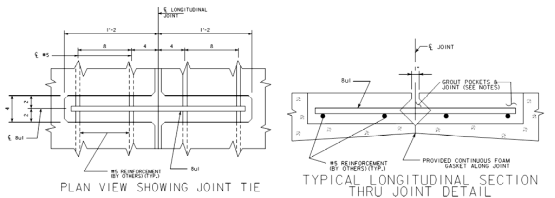
\includegraphics[max width=\textwidth]{detalhe-juntas.png}
	\end{center}
	\fonte{\citeonline[p.~15]{Rouse}}
\end{figure}

\begin{figure}[htb]
	\caption{\label{grauteamento}Grauteamento das juntas longitudinais.}
	\begin{center}
		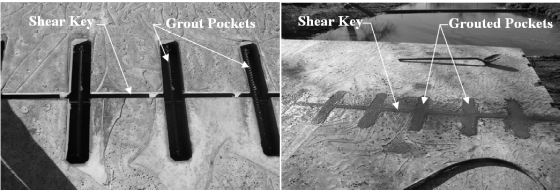
\includegraphics[max width=\textwidth]{grauteamento.png}
	\end{center}
	\fonte{\citeonline[p.~15]{Rouse}}
\end{figure}

\begin{figure}[htb]
	\caption{\label{protensao}Detalhe da protensão.}
	\begin{center}
		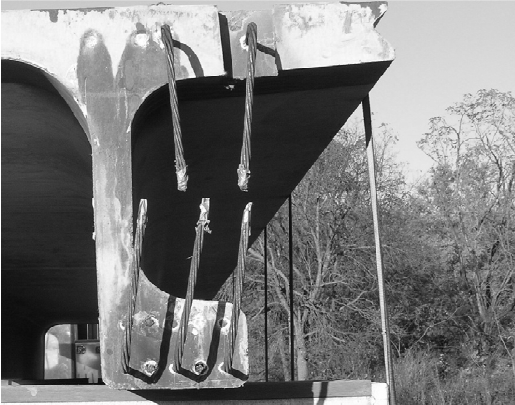
\includegraphics[max width=\textwidth]{protensao.png}
	\end{center}
	\fonte{\citeonline[p.~16]{Rouse}}
\end{figure}

% % %

\begin{figure}[htb]
	\caption{\label{detalhe-diafragma}Detalhamento do diafragma.}
	\begin{center}
		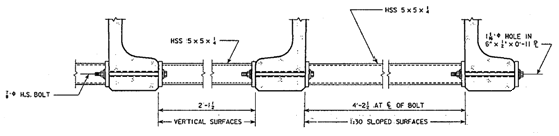
\includegraphics[max width=\textwidth]{detalhe-diafragma}
	\end{center}
	\fonte{\citeonline[p.~14]{Rouse}}
\end{figure}

\begin{figure}[htb]
	\caption{\label{foto-diafragma}Diafragma instalado entre as vigas de uma mesma seção e entre as vigas de seções adjacentes.}
	\begin{center}
		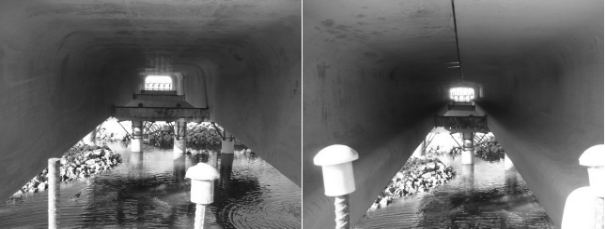
\includegraphics[max width=\textwidth]{foto-diafragma.png}
	\end{center}
	\fonte{\citeonline[p.~14]{Rouse}}
\end{figure}

\begin{figure}[htb]
	\caption{\label{instalacao}Instalação dos elementos estruturais.}
	\begin{center}
		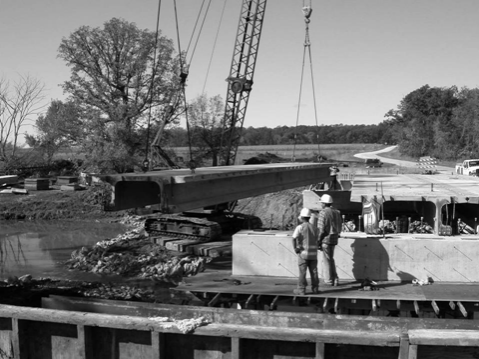
\includegraphics[max width=\textwidth]{instalacao.png}
	\end{center}
	\fonte{\citeonline[p.~18]{Rouse}}
\end{figure}

\begin{figure}[htb]
	\caption{\label{jakway-park}Ponte Jakway Park. Apenas o trecho do vão central é feito de CUAD.}
	\begin{center}
		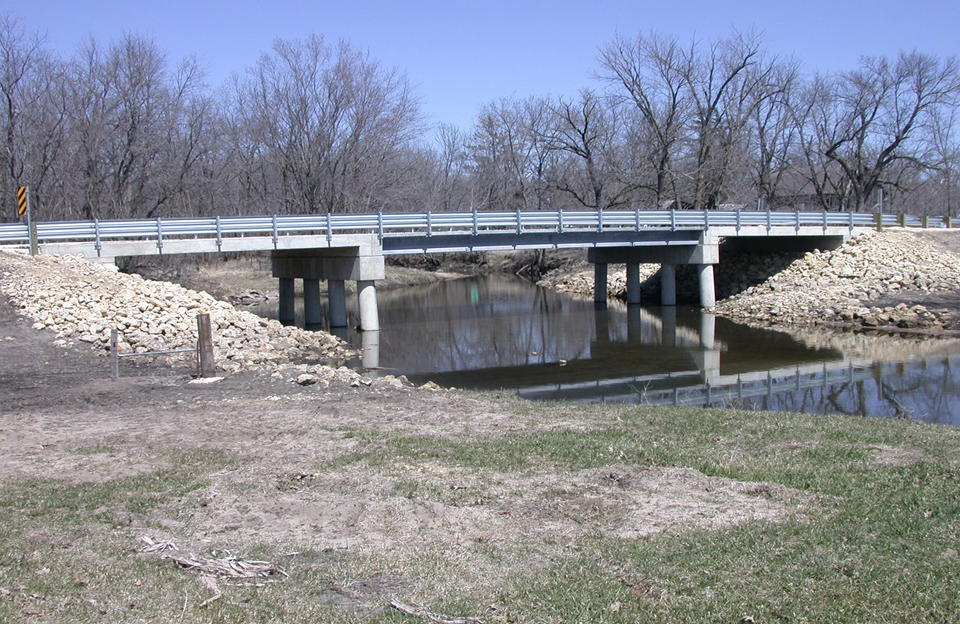
\includegraphics[max width=\textwidth]{jakway-park.png}
	\end{center}
	\fonte{\citeonline{Keierleber_email}}
\end{figure}

%2nd preceedings 579 Design of First Hybrid UHPC-Steel Bridge across the River
%Fulda in Kassel, Germany